\section{Logic Analyzer Results}
After completing the DC sweep, students were instructed to use a zero to five
volt ramp function at~\SI{10}{\hertz} as the system's input.  While the system
counted from~0 to~255 more quickly than could be observed by the naked eye,
students used the in-lab logic analyzer to observe the signal on the pin
labeled~$\overline{\text{INTR}}$.  This signal can be seen below in
Figure~\ref{f:intr}.
%
\begin{figure}[H]
\centering
	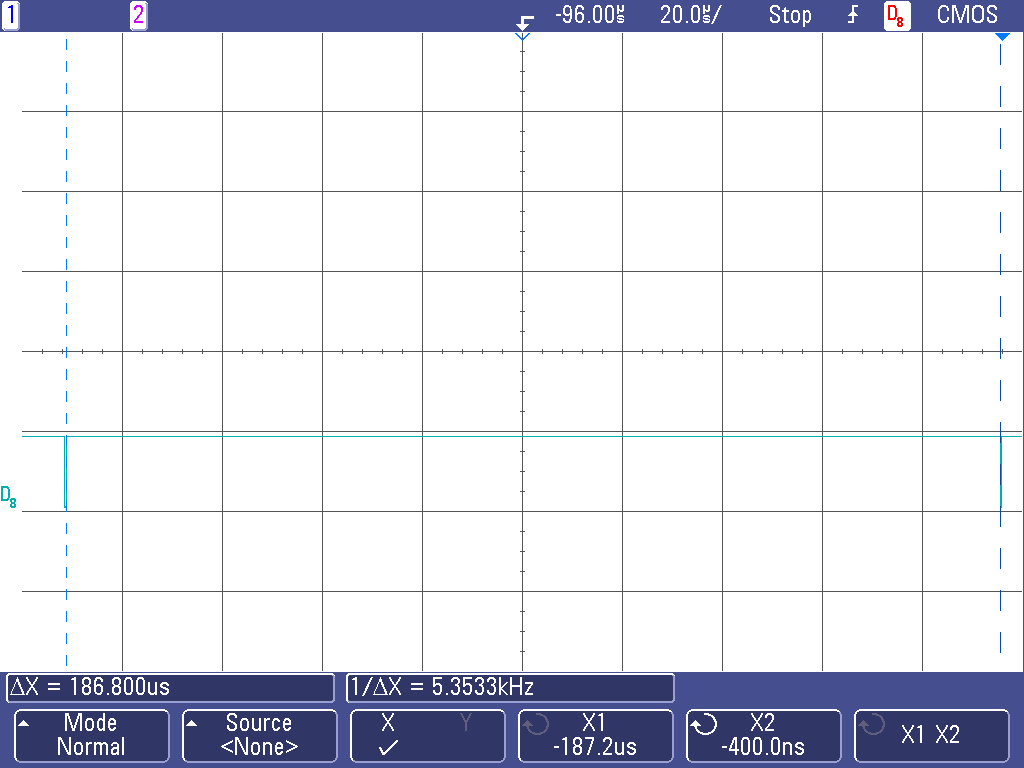
\includegraphics[width=.8\textwidth]{img/shot/intr_high_period.png}
	\parbox{.8\textwidth}{
	\caption[\texttt{INTR\_} Waveform]{Logic analyzer capture of the pin
	labeled \texttt{INTR\_} for a~\SI{10}{\hertz} input ramp function from zero
	to five volts.}
	\label{f:intr}}
\end{figure}
%
The $\overline{\text{INTR}}$ pin is normally high~(\SI{5}{\volt}) and
momentarily drops to ground when a measurement has been completed.  In the
displayed subset of captured measurements,~\SI{186.6}{\micro\second} pass
between the two pulses.  By utilizing the clock frequency calculated earlier in
step two, the number of clock cycles that pass while
the~$\overline{\text{INTR}}$ pin is high can be calculated.
%
\begin{align}
	\text{\# Clock Cycles} &= f_\text{clock} \cdot t_{\overline{\text{INTR}}\text{ HI}}\label{eq:clock_cycles}\\
	&= \SI{379}{\kilo\hertz} \cdot \SI{186.6}{\micro\second}\nonumber \\
	&= \SI{70.72}{Cycles} \nonumber
\end{align}
%
As is shown by~\eqref{eq:clock_cycles}, roughly seventy clock cycles pass
between pulses on~$\overline{\text{INTR}}$, and thus between each reading.  The
datasheet for the Harris ADC0804 IC indicates that~64 cycles are required for
complete reading --- six cycles fewer than were observed.  Coincidentally, in a
previous experiment with this ADC an extra six cycles were allocated to the
reset process.  By applying those six cycles to the datasheet's listed value,
the observed behavior is correct: it took roughly~70 cycles to complete a
conversion from analog to digital.
